% ============================================================================
%  Capstone Report: RDMA-Accelerated Distributed LLM Inference
%  Single-file LaTeX source. Paste into a blank Overleaf project and compile
%  with pdfLaTeX. No external figures or .bib file required.
% ============================================================================
\documentclass[11pt,a4paper]{article}

\usepackage[margin=1in]{geometry}
\usepackage[T1]{fontenc}
\usepackage{lmodern}
\usepackage{amsmath,amssymb}
\usepackage{booktabs}
\usepackage{tabularx}
\usepackage{longtable}
\usepackage{xcolor}
\usepackage{listings}
\usepackage{tikz}
\usetikzlibrary{arrows.meta,positioning,fit,calc}
\usepackage{enumitem}
\usepackage{caption}
\usepackage[hidelinks]{hyperref}

\definecolor{codebg}{RGB}{246,248,250}
\definecolor{todo}{RGB}{200,30,30}
\newcommand{\TODO}[1]{\textcolor{todo}{\textbf{[TODO: #1]}}}

\lstset{
  basicstyle=\ttfamily\footnotesize,
  backgroundcolor=\color{codebg},
  frame=single, rulecolor=\color{gray!40},
  breaklines=true, columns=fullflexible,
  keywordstyle=\color{blue!60!black}\bfseries,
  commentstyle=\color{green!40!black},
  showstringspaces=false
}

\title{\textbf{RDMA-Accelerated Pipeline-Parallel Inference\\for Large Language Models on a Virtualised Soft-RoCE Cluster}}
\author{Dishanth Arya\\ \small Capstone Project Report}
\date{\today}

\begin{document}
\maketitle

\begin{abstract}
Large Language Models (LLMs) such as Qwen2.5-7B no longer fit comfortably in the memory of a single commodity machine. A common answer is \emph{pipeline parallelism}: the transformer's decoder layers are split across several nodes, and each node forwards its intermediate hidden-state tensor to the next. This makes the network link between stages a first-class part of inference latency. This project builds a working multi-node pipeline-parallel inference system in which hidden states move between nodes through \emph{Remote Direct Memory Access} (RDMA) one-sided writes instead of the TCP/IP socket stack. The system is built on Soft-RoCE (\texttt{rdma\_rxe}) so that it runs on ordinary Ethernet and inside QEMU/KVM virtual machines. It consists of (i) a C ``bridge'' that registers a POSIX shared-memory mailbox with the RDMA NIC and forwards tensors with \texttt{IBV\_WR\_RDMA\_WRITE}, (ii) a PyTorch runtime that slices Qwen2.5-7B by layer and talks to the bridge through the shared mailbox, (iii) a telemetry-driven layer arbitrator that splits layers in proportion to each node's free memory, and (iv) a reproducible QEMU cluster of 2--5 nodes with a benchmark suite that compares RDMA and TCP on time-to-first-token (TTFT), inter-token latency (ITL) and throughput.
\end{abstract}

\tableofcontents
\newpage

% ============================================================================
\section{Introduction}
% ============================================================================

\subsection{Motivation}
Autoregressive LLM inference produces one token at a time. Each token requires a full forward pass through every decoder layer. When the model is split across $N$ machines, every forward pass crosses $N-1$ network hops (plus one return hop for the generated token). Two phases stress the network differently:
\begin{itemize}[leftmargin=*]
  \item \textbf{Prefill} (first token). The whole prompt of $L$ tokens is processed at once. The hidden state sent between stages has shape $[1, L, 3584]$ in FP32, i.e.\ $L \times 3584 \times 4$ bytes. For $L=1024$ that is about 14.7\,MB per hop.
  \item \textbf{Decode} (every later token). Without a KV cache the tensor grows by one row per step; with a cache it is a single row of about 14\,KB. These are small, latency-bound messages, where per-message software overhead dominates.
\end{itemize}
In both cases the classic TCP/IP path adds kernel transitions, buffer copies and protocol processing on every hop. RDMA removes most of this: after a one-time setup, the NIC writes directly into a remote, pre-registered memory region without involving the remote CPU or kernel.

\subsection{Goals}
\begin{enumerate}[leftmargin=*]
  \item Build an end-to-end pipeline-parallel inference path for a real 7B-parameter LLM where inter-stage tensors move by one-sided RDMA writes.
  \item Make it run without RDMA hardware (Soft-RoCE over Ethernet, inside VMs), so the setup is cheap and reproducible.
  \item Allocate layers to nodes according to live resource telemetry instead of a fixed split.
  \item Compare RDMA against a TCP baseline across cluster size, prompt length and generation length.
\end{enumerate}

\subsection{Contributions}
\begin{itemize}[leftmargin=*]
  \item A \textbf{shared-memory RDMA bridge} (\texttt{rdma\_llm.c}, \texttt{rdma\_pipeline.c}) that registers a POSIX \texttt{shm} region directly as an RDMA memory region, so the Python/PyTorch process and the NIC operate on the same bytes with no extra copy in user space.
  \item A \textbf{28-byte header protocol} with a \texttt{job\_status} state machine that lets a Python process and a C process coordinate through polling on shared memory.
  \item A \textbf{telemetry-driven layer arbitrator} (\texttt{rdma\_arbitrator.c}) that reads \texttt{/proc/stat} and \texttt{/proc/meminfo}, computes a memory-proportional layer split, and pushes the decision to the peer with an RDMA write once per second.
  \item A \textbf{generalised $N$-stage pipeline} (\texttt{distributed\_pipeline.py}) with pluggable TCP and RDMA/shared-memory transports, a real Qwen2.5-7B stage and a synthetic stage for weight-free benchmarking.
  \item A \textbf{reproducible virtual cluster}: a custom minimal initramfs, a QEMU/KVM cluster manager for 2--5 nodes on a Linux bridge, a VM worker daemon, and a benchmark/plotting suite.
\end{itemize}

% ============================================================================
\section{Background}
% ============================================================================

\subsection{RDMA and the Verbs API}
RDMA lets one machine read or write another machine's memory through the NIC. The programming interface (\texttt{libibverbs}) splits work into a \emph{control path} and a \emph{data path}:
\begin{itemize}[leftmargin=*]
  \item \textbf{Control path} (slow, done once): open the device, allocate a protection domain (PD), register memory regions (MR) to obtain local/remote keys (\texttt{lkey}/\texttt{rkey}), create completion queues (CQ) and queue pairs (QP), and move each QP through the states \texttt{RESET}$\rightarrow$\texttt{INIT}$\rightarrow$\texttt{RTR}$\rightarrow$\texttt{RTS}.
  \item \textbf{Data path} (fast, per message): post a work request (\texttt{ibv\_post\_send}) and poll the CQ (\texttt{ibv\_poll\_cq}). No system call is made.
\end{itemize}
A \emph{one-sided} \texttt{RDMA\_WRITE} places data in the remote MR without any action by the remote CPU. The sender only needs the remote virtual address and \texttt{rkey}, which are exchanged once out of band.

\subsection{RoCE and Soft-RoCE}
RDMA over Converged Ethernet (RoCEv2) carries InfiniBand transport inside UDP/IP packets. \emph{Soft-RoCE} (\texttt{rdma\_rxe}) is a Linux kernel driver that implements RoCEv2 in software on any Ethernet interface. It exposes the same verbs API as a hardware RNIC, so the code in this project runs unmodified on real RoCE/InfiniBand hardware. On Soft-RoCE the protocol processing still runs on the CPU (in the kernel), so absolute gains are smaller than on hardware RNICs; the application, however, avoids socket system calls and user/kernel buffer copies.

\subsection{Pipeline Parallelism for LLMs}
A decoder-only transformer is a stack of identical layers. Pipeline parallelism assigns a contiguous range of layers to each node. Node $0$ embeds the input and runs its layers; each intermediate node receives a hidden state, runs its layers and forwards the result; the last node applies the final RMSNorm and LM head and emits a token, which is sent back to node~0 to extend the sequence.

\subsection{Target Model: Qwen2.5-7B}
\begin{table}[h]
\centering
\begin{tabular}{@{}ll@{}}
\toprule
Property & Value \\
\midrule
Architecture & \texttt{Qwen2ForCausalLM} (decoder-only) \\
Decoder layers & 28 \\
Hidden size & 3584 \\
FFN intermediate size & 18944 \\
Attention heads / KV heads & 28 / 4 (grouped-query attention) \\
Vocabulary & 152{,}064 \\
Native dtype & bfloat16 \\
\bottomrule
\end{tabular}
\caption{Model configuration (from \texttt{qwen\_weights/config.json}).}
\end{table}

% ============================================================================
\section{Related Work}
% ============================================================================
\begin{description}[leftmargin=*,style=nextline]
  \item[fabric-lib (Perplexity, MLSys 2026)] A portable RDMA point-to-point library for LLM systems that works on both NVIDIA ConnectX (RC) and AWS EFA (SRD). It relies only on \emph{reliable but unordered} delivery and adds an \texttt{ImmCounter} primitive for completion notification. Used for KV-cache transfer, 1.3\,s RL weight updates on trillion-parameter models, and MoE dispatch/combine. It supports our design choice of one-sided writes plus a lightweight completion signal instead of collectives.
  \item[OnePiece (Tencent WeChat, 2026)] Splits multi-stage AI-content-generation pipelines into microservices connected by one-sided RDMA. Introduces a double-ring buffer that avoids deadlock without CPU involvement, and a Node Manager that rebalances resources with load. Close in spirit to our shared mailbox and our arbitrator.
  \item[FARLock (OSDI 2026)] A fair RDMA distributed lock that combines ticket locks with MCS-style handover, so requests are served in arrival order while local requests avoid NIC loopback. Relevant to our polling-based \texttt{job\_status} handshake, which is currently a simple flag rather than a proper synchronisation primitive.
  \item[MDI-LLM (Macario et al., 2025)] Model-distributed LLM inference across low-power edge devices (Jetson TX2 over gigabit Ethernet) with ``recurrent pipeline parallelism'' to keep every device busy while generating several sequences. Uses TCP; it is the closest workload match to this project and shows the value of keeping the pipeline full.
  \item[Kafetzis et al.\ (2025)] Resource-aware partitioning of transformers at attention-head granularity, re-run during generation and migrating blocks when resources change. Reaches within 15--20\% of an optimal solver and up to 9--10$\times$ lower latency than layer-level partitioning in simulation. Motivates making our arbitrator finer-grained and dynamic.
\end{description}

% ============================================================================
\section{System Design}
% ============================================================================

\subsection{Architecture Overview}
\begin{figure}[h]
\centering
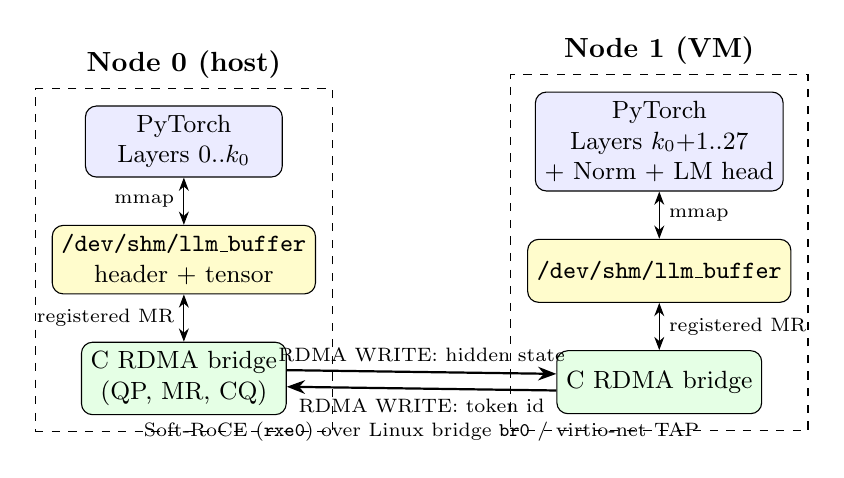
\begin{tikzpicture}[
  node distance=0.6cm and 0.9cm,
  box/.style={draw, rounded corners, minimum width=2.5cm, minimum height=0.8cm, align=center, font=\small},
  py/.style={box, fill=blue!8},
  shm/.style={box, fill=yellow!20},
  c/.style={box, fill=green!10},
  >=Stealth]
  % Node 0
  \node[py]  (py0)  {PyTorch\\Layers $0..k_0$};
  \node[shm, below=of py0] (shm0) {\texttt{/dev/shm/llm\_buffer}\\header + tensor};
  \node[c,   below=of shm0] (c0) {C RDMA bridge\\(QP, MR, CQ)};
  \node[draw, dashed, fit=(py0)(shm0)(c0), inner sep=6pt, label=above:{\textbf{Node 0 (host)}}] {};
  % Node 1
  \node[py,  right=3.2cm of py0] (py1) {PyTorch\\Layers $k_0{+}1..27$\\+ Norm + LM head};
  \node[shm, below=of py1] (shm1) {\texttt{/dev/shm/llm\_buffer}};
  \node[c,   below=of shm1] (c1) {C RDMA bridge};
  \node[draw, dashed, fit=(py1)(shm1)(c1), inner sep=6pt, label=above:{\textbf{Node 1 (VM)}}] {};
  % arrows
  \draw[<->] (py0) -- node[left,font=\scriptsize]{mmap} (shm0);
  \draw[<->] (shm0) -- node[left,font=\scriptsize]{registered MR} (c0);
  \draw[<->] (py1) -- node[right,font=\scriptsize]{mmap} (shm1);
  \draw[<->] (shm1) -- node[right,font=\scriptsize]{registered MR} (c1);
  \draw[->, thick] ([yshift=3pt]c0.east) -- node[above,font=\scriptsize]{RDMA WRITE: hidden state} ([yshift=3pt]c1.west);
  \draw[<-, thick] ([yshift=-3pt]c0.east) -- node[below,font=\scriptsize]{RDMA WRITE: token id} ([yshift=-3pt]c1.west);
  \node[below=0.4cm of $(c0)!0.5!(c1)$, font=\scriptsize, align=center] {Soft-RoCE (\texttt{rxe0}) over Linux bridge \texttt{br0} / virtio-net TAP};
\end{tikzpicture}
\caption{Two-node data path. PyTorch and the C bridge share one POSIX shared-memory region; that region is also the RDMA memory region, so the NIC reads and writes the same bytes PyTorch sees.}
\label{fig:arch}
\end{figure}

The system has three layers:
\begin{enumerate}[leftmargin=*]
  \item \textbf{Compute layer (Python/PyTorch).} Loads Qwen2.5-7B with HuggingFace \texttt{transformers}, keeps only its slice of \texttt{model.model.layers}, and replaces the final norm with \texttt{Identity} on every stage except the last so raw hidden states are forwarded.
  \item \textbf{Mailbox layer (POSIX shared memory).} A region created with \texttt{shm\_open("llm\_buffer")} and mapped by both processes.
  \item \textbf{Transport layer (C, libibverbs).} Registers the same mapping with \texttt{ibv\_reg\_mr}, connects an RC queue pair to the peer, and moves data with \texttt{IBV\_WR\_RDMA\_WRITE}.
\end{enumerate}

\subsection{Shared Mailbox Layout and Protocol}
The mailbox starts with a 28-byte header of seven \texttt{int32} fields, followed by the tensor:
\begin{lstlisting}[language=C]
struct llm_shared_pool {
    volatile int32_t job_status;        // 0 idle, 1 tensor ready, 2 token ready, 99 terminate
    volatile int32_t current_layer;
    volatile int32_t current_seq_len;
    volatile int32_t generated_token_id;
    volatile int32_t status;
    volatile int32_t total_nodes;       // host_layers in rdma_llm.c
    volatile int32_t rank;              // vm_layers  in rdma_llm.c
    // float32 tensor [1, seq_len, 3584] follows
};
#define SHARED_MEM_SIZE (28 + (1024 * 3584 * 4))   // 14,680,092 bytes
\end{lstlisting}
Python packs and unpacks the header with \texttt{struct.pack('7i', ...)}. The \texttt{volatile} qualifier forces the C polling loop to re-read memory, because the NIC can change the region at any time.

\paragraph{Two-node token loop (\texttt{rdma\_llm.c} + \texttt{distributed\_llm.py}).}
\begin{enumerate}[leftmargin=*]
  \item Host Python runs layers $0$--$23$, writes the hidden state after the header, sets \texttt{seq\_len} and \texttt{job\_status=1}.
  \item Host C bridge sees \texttt{job\_status==1}, posts one RDMA write of the whole region into the VM's mailbox, and polls the CQ for completion.
  \item VM Python sees \texttt{job\_status==1}, runs layers $24$--$27$, the final norm and the LM head, takes the arg-max token, writes it to \texttt{generated\_token\_id} and sets \texttt{job\_status=2}.
  \item VM C bridge sees \texttt{job\_status==2}, RDMA-writes the region back to the host, and resets its flag.
  \item Host Python sees \texttt{job\_status==2}, decodes the token, appends it to \texttt{input\_ids} and starts the next step.
\end{enumerate}

\subsection{Connection Setup}
Every C component uses the same out-of-band bootstrap. Each side fills a \texttt{rdma\_connection\_data} record (MR address, \texttt{rkey}, QP number, LID, GID) and swaps it over a short TCP connection. The QP is then moved to \texttt{INIT} (remote read/write allowed), \texttt{RTR} (path MTU 1024, destination QPN and GID, hop limit 1) and \texttt{RTS} (timeout 14, retry count 7). After that TCP is not used on the data path.

\subsection{Telemetry-Driven Layer Arbitration}
\texttt{rdma\_arbitrator.c} decides how many layers each node runs. During the handshake each side also sends its total RAM. The host then loops once per second:
\begin{enumerate}[leftmargin=*]
  \item Read CPU utilisation from the delta of \texttt{/proc/stat} counters and free memory from \texttt{MemAvailable} in \texttt{/proc/meminfo}.
  \item Split $T$ layers in proportion to memory:
  \[
     \ell_{\text{host}} = \left\lfloor T \cdot \frac{M_{\text{host}}^{\text{free}}}{M_{\text{host}}^{\text{free}} + M_{\text{vm}}^{\text{total}}} \right\rfloor,
     \qquad \ell_{\text{vm}} = T - \ell_{\text{host}},
  \]
  clamped so each node keeps at least one layer.
  \item Write \texttt{\{"host\_layers": ..., "vm\_layers": ...\}} to \texttt{/dev/shm/llm\_split.json} for the local PyTorch process, and RDMA-write the telemetry struct into the VM's memory so the VM sees the same decision.
\end{enumerate}

\subsection{Generalised $N$-Stage Pipeline}
\texttt{distributed\_pipeline.py} extends the two-node prototype to $N \in \{2,\dots,5\}$ ranks.
\begin{itemize}[leftmargin=*]
  \item \textbf{Layer slicing.} \texttt{get\_layer\_slice} divides 28 layers as evenly as possible; the first $28 \bmod N$ ranks get one extra layer.
  \item \textbf{Roles.} Rank 0 tokenises and runs the first slice, then waits for the token. Intermediate ranks receive, compute and forward. The last rank computes the token and sends it back to rank 0, closing a ring.
  \item \textbf{TCP transport.} Each rank listens on \texttt{port\_base+rank}, connects to its successor (the last rank connects to rank 0), and sets \texttt{TCP\_NODELAY}. Messages are a 28-byte header followed by the raw tensor.
  \item \textbf{RDMA/shared-memory transport.} Ranks read and write the header and tensor in \texttt{/dev/shm/llm\_buffer}; the companion \texttt{rdma\_pipeline.c} bridge forwards the region to the next rank with an RDMA write sized to $28 + L \cdot 3584 \cdot 4$ bytes.
  \item \textbf{Stages.} \texttt{RealPyTorchModelStage} runs real Qwen2.5-7B layers. \texttt{SyntheticModelStage} replaces each layer with a $3584 \times 3584$ matrix multiply plus normalisation, so the full pipeline and its network traffic can be benchmarked without the 15\,GB of weights.
  \item \textbf{Metrics.} Rank 0 records per-step compute, send and wait times and writes a JSON summary: TTFT, ITL mean/std/P50/P90/P99, decode tokens/s, compute vs.\ network time and effective prefill bandwidth.
\end{itemize}

% ============================================================================
\section{Implementation and Infrastructure}
% ============================================================================

\subsection{Code Map}
\begin{table}[h]
\centering
\small
\begin{tabularx}{\linewidth}{@{}lrX@{}}
\toprule
File & LOC & Purpose \\
\midrule
\texttt{capstone/rdma/rdma\_compute.c} & 160 & First proof of concept: host writes a vector into the VM by RDMA, VM multiplies by 10 and writes back. \\
\texttt{capstone/rdma/rdma\_arbitrator.c} & 308 & Live CPU/RAM telemetry, memory-proportional layer split, RDMA push of the decision. \\
\texttt{capstone/rdma/rdma\_llm.c} & 228 & Two-node RDMA bridge over a 14\,MB shared-memory mailbox. \\
\texttt{capstone/rdma/rdma\_pipeline.c} & 267 & $N$-rank bridge with \texttt{--rank}, \texttt{--total-nodes}, \texttt{--downstream-ip}; size-aware writes. \\
\texttt{capstone/rdma/distributed\_llm.py} & 147 & Two-node Qwen2.5-7B inference (host layers 0--23, VM layers 24--27). \\
\texttt{capstone/rdma/distributed\_pipeline.py} & 618 & $N$-stage pipeline, TCP and RDMA transports, real and synthetic stages, metrics. \\
\texttt{capstone/rdma/vm\_worker.py} & 111 & HTTP daemon in each VM (\texttt{/health}, \texttt{/start}, \texttt{/status}, \texttt{/stop}) that launches a pipeline stage. \\
\texttt{scripts/cluster\_mgr.sh} & 319 & Creates bridge \texttt{br0}, TAP devices and host \texttt{rxe0}; boots 2--5 QEMU/KVM VMs. \\
\texttt{scripts/repack\_initramfs.sh} & 31 & Rebuilds the VM initramfs from \texttt{initfs/}. \\
\texttt{initfs/init} & 106 & VM boot script: mounts, IP from \texttt{vm\_id}, Soft-RoCE, 9p weights share, worker daemon. \\
\texttt{experiments/rigorous\_benchmark.py} & 525 & Parameter sweep with warm-up, trials, 95\% CI, checkpoint/resume. \\
\texttt{experiments/plot\_rigorous\_results.py} & 390 & Publication-style figures and a Markdown summary. \\
\bottomrule
\end{tabularx}
\caption{Main source files.}
\end{table}

\subsection{Virtual Cluster}
\begin{itemize}[leftmargin=*]
  \item \textbf{Kernel and initramfs.} A custom \texttt{bzImage} with \texttt{rdma\_rxe} and \texttt{ib\_uverbs}, plus a BusyBox initramfs carrying \texttt{libibverbs}, the \texttt{rxe} provider, \texttt{rdma}, \texttt{ibv\_devinfo} and \texttt{ibv\_rc\_pingpong}.
  \item \textbf{Boot.} QEMU passes \texttt{vm\_id} and \texttt{total\_nodes} on the kernel command line. \texttt{/init} assigns \texttt{192.168.100.(vm\_id+1)}, runs \texttt{rdma link add rxe0 type rxe netdev eth0}, creates \texttt{/dev/infiniband/uverbs0} from sysfs, and mounts a 2\,GB \texttt{tmpfs} on \texttt{/dev/shm}.
  \item \textbf{Weights and Python.} The host's \texttt{qwen\_weights} directory (weights, a Python environment and the pipeline scripts) is shared into every VM read-only through virtio-9p at \texttt{/mnt/weights}, so the 15\,GB model is not copied per VM.
  \item \textbf{Network.} Each VM gets a TAP device on bridge \texttt{br0} (\texttt{192.168.100.1/24}); the host also binds \texttt{rxe0} to \texttt{br0} so it can act as rank 0.
  \item \textbf{Orchestration.} The benchmark waits for each VM's \texttt{/health} endpoint, then sends \texttt{POST /start} with rank, node list and backend.
\end{itemize}

\subsection{Benchmark Methodology}
\texttt{rigorous\_benchmark.py} sweeps four factors:
\begin{table}[h]
\centering
\begin{tabular}{@{}llll@{}}
\toprule
Factor & quick & standard & full \\
\midrule
Nodes $N$ & 2,3,4,5 & 2,3,4,5 & 2,3,4,5 \\
Prompt length (tokens) & 32, 256 & 32, 256, 1024 & 32, 128, 512, 1024 \\
Generated tokens & 10, 25 & 10, 50, 100 & 10, 25, 50, 100 \\
Backend & TCP, RDMA & TCP, RDMA & TCP, RDMA \\
\bottomrule
\end{tabular}
\caption{Benchmark profiles. Prefill payload per hop ranges from about 0.46\,MB (32 tokens) to 14.7\,MB (1024 tokens).}
\end{table}

Each cell runs warm-up iterations and several trials. The suite reports mean, standard deviation and 95\% confidence interval ($1.96\,\sigma/\sqrt{n}$) for TTFT, mean ITL, P50/P90/P99 ITL, decode tokens/s, and the compute/network split, plus ITL speed-up $= \text{ITL}_{\text{TCP}} / \text{ITL}_{\text{RDMA}}$. It runs in \emph{local} mode (all ranks as processes on one machine) or \emph{cluster} mode (rank 0 on the host, other ranks in VMs).

% ============================================================================
\section{Results}

\subsection{Setup}
The sweep used the \emph{standard} profile (nodes $N \in \{2,3,4,5\}$, prompt lengths 32/256/1024 tokens, 10/50/100 generated tokens, TCP and RDMA backends): 72 configurations in 2402.3\,s of wall time. All runs used the synthetic model stage (\texttt{--benchmark}), so the compute per layer is a $3584 \times 3584$ matrix multiply, not a real Qwen layer. The RDMA backend returned results, which is only possible in \emph{local} mode (the default since commit \texttt{efa8895}): in cluster mode the RDMA transport has no bridge process and the stages cannot reach each other. All numbers below therefore come from processes on one machine, where ``TCP'' is loopback sockets and ``RDMA'' is the shared-memory mailbox.

\subsection{Headline Numbers}
\begin{table}[h]
\centering
\small
\begin{tabular}{@{}ccccccc@{}}
\toprule
$N$ & Prompt & Backend & TTFT (ms) & ITL mean (ms) & ITL P99 (ms) & tok/s \\
\midrule
2 & 32   & TCP  & 25.7 & 27.73 & 29.77 & 36.1 \\
2 & 32   & RDMA & 24.8 & 25.70 & 26.84 & 38.9 \\
2 & 256  & TCP  & 34.0 & 32.38 & 33.63 & 30.9 \\
2 & 256  & RDMA & 28.2 & 29.72 & 31.38 & 33.6 \\
2 & 1024 & TCP  & 47.0 & 45.34 & 47.14 & 22.1 \\
2 & 1024 & RDMA & 39.2 & 38.51 & 40.55 & 26.0 \\
\midrule
5 & 1024 & TCP  & 99.2 & 89.51 & 109.84 & 11.2 \\
5 & 1024 & RDMA & 28.9 & 17.05 & 33.59  & 58.7 \\
\bottomrule
\end{tabular}
\caption{Selected results, 100 generated tokens. The full 72-row table is in Appendix~\ref{app:results}. The $N=5$ RDMA row is \emph{not} a valid pipeline measurement (Section~\ref{sec:validity}).}
\label{tab:headline}
\end{table}

\begin{table}[h]
\centering
\small
\begin{tabular}{@{}ccccc@{}}
\toprule
$N$ & Mean ITL, TCP (ms) & Mean ITL, RDMA (ms) & ITL speed-up range & Valid? \\
\midrule
2 & 34.63 & 30.93 & 1.04--1.18$\times$ & Yes (local IPC vs.\ loopback) \\
3 & 40.96 & 17.36 & 1.80--2.85$\times$ & No \\
4 & 46.35 & 15.08 & 2.31--3.38$\times$ & No \\
5 & 53.38 & 12.59 & 3.28--5.25$\times$ & No \\
\bottomrule
\end{tabular}
\caption{Mean ITL averaged over all prompt and generation lengths for each cluster size.}
\label{tab:byN}
\end{table}

\subsection{Findings}
\begin{enumerate}[leftmargin=*]
  \item \textbf{Two nodes: the shared-memory path is 4--18\% faster than TCP.} At $N=2$ there is one producer and one consumer, so the mailbox protocol is correct. RDMA-backend ITL is lower in all 9 configurations, with speed-up 1.04--1.08$\times$ at 32 tokens, 1.09--1.13$\times$ at 256 tokens, and 1.15--1.18$\times$ at 1024 tokens. TTFT falls from 47.0--48.3\,ms to 38.8--39.2\,ms at 1024 tokens. The gain grows with payload size, which matches the expected cost of copying a 14.7\,MB tensor through the socket stack. P99 ITL is also lower in every case.
  \item \textbf{TCP behaves like a correct pipeline.} With TCP, more nodes mean more hops for the same 28 layers of compute, so latency should rise with $N$. It does: mean ITL grows from 34.63\,ms ($N=2$) to 53.38\,ms ($N=5$), and at 1024 tokens TTFT roughly doubles, from 47.0\,ms to 99.2\,ms. Larger prompts also cost more per hop: at $N=5$, ITL rises from 28.62\,ms (32 tokens) to 84.42\,ms (1024 tokens).
  \item \textbf{The RDMA backend gets faster as nodes are added, which a pipeline cannot do.} RDMA mean ITL \emph{falls} from 30.93\,ms ($N=2$) to 12.59\,ms ($N=5$), and throughput rises to 120\,tok/s. Total compute per token is fixed at 28 layers and every extra node adds a hop, so a correct pipeline cannot speed up this way. The reported 1.8--5.25$\times$ speed-ups for $N \ge 3$ are an artefact, explained next.
\end{enumerate}

\subsection{Validity of the $N \ge 3$ RDMA Results}
\label{sec:validity}
In local mode every rank maps the same file, \texttt{/dev/shm/llm\_buffer}. Every non-zero rank polls the same \texttt{job\_status} field and accepts any header with \texttt{job\_status==1}, so whichever rank polls first takes the tensor. To check this, the pipeline was re-run with $N=3$, 32-token prompt and 10 generated tokens, with a log line each time a rank picked up a tensor (\texttt{header[6]} holds the sender's rank):

\begin{table}[h]
\centering
\small
\begin{tabular}{@{}lcc@{}}
\toprule
Event & Rank 1 & Rank 2 (final) \\
\midrule
Took tensor from rank 0 & 1 & 1 \\
Took tensor from rank 1 & 6 & 3 \\
\bottomrule
\end{tabular}
\caption{Which rank consumed which tensor in a 3-node local RDMA run.}
\end{table}

The final rank took a tensor directly from rank 0, so rank 1's layers were \emph{skipped} for that token. Rank 1 also picked up its \emph{own} output six times and processed it again. The number of stages that run per token is therefore random, and with more ranks the final rank is more likely to win the race early, with less compute done. This explains why RDMA ``speed-up'' grows with $N$. Only the $N=2$ RDMA results are valid, and even these compare local shared memory with loopback TCP, not RDMA over a network.

\subsection{What Can Be Claimed}
\begin{itemize}[leftmargin=*]
  \item A copy-free shared-memory hand-off between pipeline stages cuts per-token latency by 4--18\% compared with loopback TCP for a two-stage pipeline, and the benefit grows with tensor size.
  \item The TCP pipeline's latency grows linearly with stage count and prompt size, as expected.
  \item No network RDMA speed-up has been measured yet. That needs the fixes in Section~\ref{sec:limits} and a cluster-mode run.
\end{itemize}

\paragraph{Qualitative result.} The two-node path (\texttt{rdma\_llm.c} + \texttt{distributed\_llm.py}) generates coherent text from Qwen2.5-7B with layers 0--23 on the host and 24--27 in a VM, with each token's hidden state crossing the Soft-RoCE link by RDMA write. \TODO{Add a sample prompt/response and a screenshot of the two terminals.}

% ============================================================================
\section{Discussion and Limitations}
\label{sec:limits}
% ============================================================================
A careful reading of the code shows several points that must be fixed or stated before the RDMA vs.\ TCP numbers can be claimed as a fair comparison.

\begin{enumerate}[leftmargin=*]
  \item \textbf{The benchmark's ``RDMA'' backend does not yet use the network.} In \texttt{distributed\_pipeline.py} the RDMA transport only reads and writes the local file \texttt{/dev/shm/llm\_buffer}. The C bridge \texttt{rdma\_pipeline} is copied into the shared folder by \texttt{cluster\_mgr.sh}, but nothing starts it. In local mode every rank maps the \emph{same} file, so ``RDMA'' measures in-memory IPC, while ``TCP'' measures loopback sockets. In cluster mode, without the bridge, the stages cannot reach each other. The bridge must be launched on every rank before RDMA results are meaningful. The benchmark in Section~\ref{sec:validity} was run in this local mode.
  \item \textbf{One mailbox for $N$ stages.} With $N>2$ in local mode, all ranks poll the same header and race to consume \texttt{job\_status==1}. This was confirmed experimentally (Section~\ref{sec:validity}): stages are skipped or repeated, which makes the $N \ge 3$ RDMA numbers invalid. Each rank needs its own buffer (for example \texttt{llm\_buffer\_<rank>}) and must accept only headers from its predecessor.
  \item \textbf{Chain wiring in \texttt{rdma\_pipeline.c}.} Only rank 0 acts as a TCP server (on \texttt{port\_base}). Rank $r>0$ connects to \texttt{port\_base}$+(r-1)$, so rank 2 and above wait for servers that never start. Each rank also creates only one QP, but a middle stage needs two: one to the previous stage and one to the next.
  \item \textbf{Polling synchronisation.} Coordination is a \texttt{volatile} flag polled every 0.25--1\,ms by both Python and C. There are no memory barriers, and the header and tensor travel in one write, so the receiver can in principle see the new flag before the full tensor. Sleeping in the poll loop also adds up to 1\,ms per hop, which can hide the RDMA advantage on small decode messages. Using \texttt{RDMA\_WRITE\_WITH\_IMM} (as in fabric-lib) or writing the flag in a second, ordered write would fix both.
  \item \textbf{No KV cache.} Each decode step re-runs the whole growing sequence, and the full $[1, L, 3584]$ tensor is re-sent every step. This inflates both compute and network time compared with a production engine.
  \item \textbf{Arbitrator not connected.} \texttt{rdma\_arbitrator.c} writes \texttt{/dev/shm/llm\_split.json}, but the pipeline uses a fixed or even split. The arbitrator also assumes 32 layers, while Qwen2.5-7B has 28, and it compares host \emph{free} RAM with VM \emph{total} RAM.
  \item \textbf{Soft-RoCE on one host.} All VMs share one physical CPU and one bridge. Soft-RoCE does its protocol work on the CPU, so results show software-overhead savings, not hardware-NIC performance.
  \item \textbf{Robustness.} Most verbs calls are not checked for errors, and the TCP handshake assumes a single \texttt{read} returns the whole struct.
\end{enumerate}

% ============================================================================
\section{Future Work}
% ============================================================================
\begin{itemize}[leftmargin=*]
  \item Launch \texttt{rdma\_pipeline} on every rank from \texttt{vm\_worker.py}, give each rank its own mailbox and two QPs, and re-run the full sweep.
  \item Replace flag polling with \texttt{RDMA\_WRITE\_WITH\_IMM} and blocking completion channels, or an ordered flag write after the payload.
  \item Add a KV cache so decode messages shrink to a single 14\,KB row.
  \item Feed the arbitrator's split into the pipeline, include CPU and link bandwidth in the cost model, and support re-partitioning during generation (following Kafetzis et al.).
  \item Overlap stages for several concurrent prompts (recurrent pipeline parallelism from MDI-LLM) to remove pipeline bubbles.
  \item Repeat the experiments on hardware RoCE/InfiniBand NICs.
\end{itemize}

% ============================================================================
\section{Conclusion}
% ============================================================================
This project delivers a complete, reproducible stack for pipeline-parallel LLM inference over RDMA on commodity hardware: a Soft-RoCE virtual cluster, a C bridge that turns a POSIX shared-memory region into an RDMA target so PyTorch and the NIC share one buffer, a telemetry-based layer arbitrator, and an $N$-stage pipeline with a TCP baseline and a statistical benchmark suite. The two-node system already runs real Qwen2.5-7B inference across a host and a VM with RDMA moving every hidden state. In a 72-configuration sweep, the copy-free shared-memory hand-off beat loopback TCP by 4--18\% in the two-stage pipeline, with the gain growing with tensor size. The larger speed-ups reported for three or more stages come from a mailbox race that skips stages, so they are not a valid result. The remaining work, listed in the previous two sections, is to give each rank its own mailbox, wire the multi-rank RDMA bridge into the benchmark, and measure the RDMA vs.\ TCP comparison end to end over the network.

% ============================================================================
\appendix
\section{Full Benchmark Results}
\label{app:results}
All 72 configurations. Speed-up is $\text{ITL}_{\text{TCP}} / \text{ITL}_{\text{RDMA}}$. RDMA rows with $N \ge 3$ are affected by the mailbox race (Section~\ref{sec:validity}) and are not valid pipeline measurements.

{\small
\begin{longtable}{@{}ccclrrrrr@{}}
\toprule
$N$ & Prompt & Gen & Backend & TTFT (ms) & ITL (ms) & P99 (ms) & tok/s & Speed-up \\
\midrule
\endfirsthead
\toprule
$N$ & Prompt & Gen & Backend & TTFT (ms) & ITL (ms) & P99 (ms) & tok/s & Speed-up \\
\midrule
\endhead
\bottomrule
\endfoot
2 & 32 & 10 & TCP & 25.6 & 25.93 & 26.24 & 38.6 & 1.00$\times$ \\
2 & 32 & 10 & \textbf{RDMA} & 24.6 & 24.86 & 25.25 & 40.2 & 1.04$\times$ \\
2 & 32 & 50 & TCP & 25.6 & 27.06 & 28.28 & 37.0 & 1.00$\times$ \\
2 & 32 & 50 & \textbf{RDMA} & 24.7 & 25.27 & 26.08 & 39.6 & 1.07$\times$ \\
2 & 32 & 100 & TCP & 25.7 & 27.73 & 29.77 & 36.1 & 1.00$\times$ \\
2 & 32 & 100 & \textbf{RDMA} & 24.8 & 25.70 & 26.84 & 38.9 & 1.08$\times$ \\
\midrule
2 & 256 & 10 & TCP & 32.8 & 32.15 & 32.86 & 31.1 & 1.00$\times$ \\
2 & 256 & 10 & \textbf{RDMA} & 28.2 & 28.39 & 28.88 & 35.2 & 1.13$\times$ \\
2 & 256 & 50 & TCP & 34.3 & 32.84 & 33.89 & 30.5 & 1.00$\times$ \\
2 & 256 & 50 & \textbf{RDMA} & 28.5 & 29.19 & 30.06 & 34.3 & 1.13$\times$ \\
2 & 256 & 100 & TCP & 34.0 & 32.38 & 33.63 & 30.9 & 1.00$\times$ \\
2 & 256 & 100 & \textbf{RDMA} & 28.2 & 29.72 & 31.38 & 33.6 & 1.09$\times$ \\
\midrule
2 & 1024 & 10 & TCP & 48.3 & 43.62 & 44.24 & 22.9 & 1.00$\times$ \\
2 & 1024 & 10 & \textbf{RDMA} & 38.8 & 37.96 & 39.65 & 26.3 & 1.15$\times$ \\
2 & 1024 & 50 & TCP & 48.1 & 44.63 & 46.19 & 22.4 & 1.00$\times$ \\
2 & 1024 & 50 & \textbf{RDMA} & 39.2 & 38.77 & 40.45 & 25.8 & 1.15$\times$ \\
2 & 1024 & 100 & TCP & 47.0 & 45.34 & 47.14 & 22.1 & 1.00$\times$ \\
2 & 1024 & 100 & \textbf{RDMA} & 39.2 & 38.51 & 40.55 & 26.0 & 1.18$\times$ \\
\midrule
3 & 32 & 10 & TCP & 27.6 & 26.81 & 27.27 & 37.3 & 1.00$\times$ \\
3 & 32 & 10 & \textbf{RDMA} & 17.2 & 14.93 & 15.70 & 67.0 & 1.80$\times$ \\
3 & 32 & 50 & TCP & 28.2 & 28.85 & 30.61 & 34.7 & 1.00$\times$ \\
3 & 32 & 50 & \textbf{RDMA} & 17.6 & 14.91 & 15.86 & 67.1 & 1.93$\times$ \\
3 & 32 & 100 & TCP & 27.3 & 29.90 & 33.15 & 33.4 & 1.00$\times$ \\
3 & 32 & 100 & \textbf{RDMA} & 17.7 & 14.85 & 15.82 & 67.4 & 2.01$\times$ \\
\midrule
3 & 256 & 10 & TCP & 41.5 & 37.65 & 38.50 & 26.6 & 1.00$\times$ \\
3 & 256 & 10 & \textbf{RDMA} & 21.5 & 16.40 & 20.08 & 61.0 & 2.30$\times$ \\
3 & 256 & 50 & TCP & 39.3 & 36.93 & 38.04 & 27.1 & 1.00$\times$ \\
3 & 256 & 50 & \textbf{RDMA} & 21.3 & 16.08 & 20.06 & 62.2 & 2.30$\times$ \\
3 & 256 & 100 & TCP & 40.4 & 37.99 & 40.93 & 26.3 & 1.00$\times$ \\
3 & 256 & 100 & \textbf{RDMA} & 21.6 & 16.07 & 19.81 & 62.2 & 2.36$\times$ \\
\midrule
3 & 1024 & 10 & TCP & 65.1 & 55.61 & 56.54 & 18.0 & 1.00$\times$ \\
3 & 1024 & 10 & \textbf{RDMA} & 36.2 & 21.34 & 27.95 & 46.9 & 2.61$\times$ \\
3 & 1024 & 50 & TCP & 65.0 & 56.95 & 61.68 & 17.6 & 1.00$\times$ \\
3 & 1024 & 50 & \textbf{RDMA} & 36.0 & 21.34 & 32.68 & 47.0 & 2.67$\times$ \\
3 & 1024 & 100 & TCP & 65.2 & 57.98 & 63.30 & 17.2 & 1.00$\times$ \\
3 & 1024 & 100 & \textbf{RDMA} & 40.9 & 20.31 & 30.11 & 49.2 & 2.85$\times$ \\
\midrule
4 & 32 & 10 & TCP & 28.6 & 27.29 & 27.92 & 36.7 & 1.00$\times$ \\
4 & 32 & 10 & \textbf{RDMA} & 13.3 & 11.80 & 12.73 & 84.7 & 2.31$\times$ \\
4 & 32 & 50 & TCP & 28.5 & 28.61 & 30.82 & 35.0 & 1.00$\times$ \\
4 & 32 & 50 & \textbf{RDMA} & 13.5 & 10.53 & 16.71 & 95.6 & 2.72$\times$ \\
4 & 32 & 100 & TCP & 28.4 & 30.72 & 35.05 & 32.6 & 1.00$\times$ \\
4 & 32 & 100 & \textbf{RDMA} & 13.7 & 11.07 & 19.07 & 90.5 & 2.78$\times$ \\
\midrule
4 & 256 & 10 & TCP & 45.9 & 40.17 & 40.61 & 25.0 & 1.00$\times$ \\
4 & 256 & 10 & \textbf{RDMA} & 17.4 & 14.15 & 17.51 & 71.3 & 2.84$\times$ \\
4 & 256 & 50 & TCP & 47.9 & 44.01 & 48.12 & 22.7 & 1.00$\times$ \\
4 & 256 & 50 & \textbf{RDMA} & 17.1 & 13.27 & 19.66 & 75.4 & 3.32$\times$ \\
4 & 256 & 100 & TCP & 46.7 & 42.33 & 47.64 & 23.9 & 1.00$\times$ \\
4 & 256 & 100 & \textbf{RDMA} & 17.4 & 12.67 & 18.21 & 79.2 & 3.34$\times$ \\
\midrule
4 & 1024 & 10 & TCP & 86.1 & 66.42 & 67.50 & 15.1 & 1.00$\times$ \\
4 & 1024 & 10 & \textbf{RDMA} & 42.7 & 21.30 & 37.45 & 46.9 & 3.12$\times$ \\
4 & 1024 & 50 & TCP & 83.5 & 68.00 & 75.17 & 14.7 & 1.00$\times$ \\
4 & 1024 & 50 & \textbf{RDMA} & 31.8 & 20.14 & 34.98 & 49.9 & 3.38$\times$ \\
4 & 1024 & 100 & TCP & 85.0 & 69.62 & 83.83 & 14.4 & 1.00$\times$ \\
4 & 1024 & 100 & \textbf{RDMA} & 36.4 & 20.76 & 36.81 & 48.5 & 3.35$\times$ \\
\midrule
5 & 32 & 10 & TCP & 30.8 & 28.62 & 29.12 & 35.0 & 1.00$\times$ \\
5 & 32 & 10 & \textbf{RDMA} & 11.3 & 8.40 & 12.60 & 120.2 & 3.41$\times$ \\
5 & 32 & 50 & TCP & 29.4 & 29.05 & 31.79 & 34.4 & 1.00$\times$ \\
5 & 32 & 50 & \textbf{RDMA} & 11.1 & 8.85 & 17.16 & 113.0 & 3.28$\times$ \\
5 & 32 & 100 & TCP & 30.8 & 32.41 & 39.45 & 30.9 & 1.00$\times$ \\
5 & 32 & 100 & \textbf{RDMA} & 13.4 & 9.16 & 20.51 & 109.5 & 3.54$\times$ \\
\midrule
5 & 256 & 10 & TCP & 51.6 & 43.96 & 44.72 & 22.9 & 1.00$\times$ \\
5 & 256 & 10 & \textbf{RDMA} & 17.6 & 10.66 & 15.74 & 95.1 & 4.12$\times$ \\
5 & 256 & 50 & TCP & 54.0 & 42.74 & 46.75 & 23.4 & 1.00$\times$ \\
5 & 256 & 50 & \textbf{RDMA} & 19.6 & 12.04 & 23.24 & 83.1 & 3.55$\times$ \\
5 & 256 & 100 & TCP & 51.2 & 45.08 & 50.29 & 22.4 & 1.00$\times$ \\
5 & 256 & 100 & \textbf{RDMA} & 17.5 & 12.19 & 24.65 & 82.3 & 3.70$\times$ \\
\midrule
5 & 1024 & 10 & TCP & 105.0 & 84.42 & 88.58 & 11.8 & 1.00$\times$ \\
5 & 1024 & 10 & \textbf{RDMA} & 35.3 & 17.86 & 25.61 & 56.2 & 4.73$\times$ \\
5 & 1024 & 50 & TCP & 98.6 & 84.63 & 106.99 & 11.8 & 1.00$\times$ \\
5 & 1024 & 50 & \textbf{RDMA} & 38.7 & 17.08 & 28.71 & 58.6 & 4.95$\times$ \\
5 & 1024 & 100 & TCP & 99.2 & 89.51 & 109.84 & 11.2 & 1.00$\times$ \\
5 & 1024 & 100 & \textbf{RDMA} & 28.9 & 17.05 & 33.59 & 58.7 & 5.25$\times$ \\
\end{longtable}
}

% ============================================================================
\begin{thebibliography}{9}
\bibitem{fabriclib} N.~Licker, K.~Hu, V.~Zaytsev, L.~Chen. \emph{fabric-lib: RDMA Point-to-Point Communication for LLM Systems}. MLSys 2026. arXiv:2510.27656.
\bibitem{onepiece} J.~Chen, N.~Xu, G.~Huang, B.~Zhou, S.~Liu. \emph{OnePiece: A Large-Scale Distributed Inference System with RDMA for Complex AI-Generated Content (AIGC) Workflows}. arXiv:2601.20655, 2026.
\bibitem{farlock} Y.~Hu, J.~Zhou, T.~Wang, K.~Vora. \emph{FARLock: Asymmetric RDMA Locking Made Fair}. USENIX OSDI 2026.
\bibitem{mdillm} D.~Macario, H.~Seferoglu, E.~Koyuncu. \emph{Model-Distributed Inference for Large Language Models at the Edge}. arXiv:2505.18164, 2025.
\bibitem{kafetzis} D.~Kafetzis, R.~Khalili, I.~Koutsopoulos. \emph{Large Language Model Partitioning for Low-Latency Inference at the Edge}. arXiv:2505.02533, 2025.
\bibitem{qwen} Qwen Team. \emph{Qwen2.5 Technical Report}. arXiv:2412.15115, 2024.
\bibitem{kalia} A.~Kalia, M.~Kaminsky, D.~G.~Andersen. \emph{Design Guidelines for High Performance RDMA Systems}. USENIX ATC 2016.
\end{thebibliography}

\end{document}
